\subsection{Catalog Completeness, Effectiveness and Reliability}
\label{s:candr}

To evaluate the performance of the Robovetter and to measure the catalog completeness and reliability, we run the Robovetter on the \injtce{s}, \invtce{s} and \scrtce{s}. 

As a high level summary, we include Figure~\ref{f:scoregrid} which provides the completeness, in-effectiveness ($1-E$) and reliability  for a 3 by 3 grid across period and MES. If the same figure is made for only the FGK dwarf type stars (surface gravity greater than or equal to $4.0$ and stellar effective temperature between $4000$ and $7000$\,K), the long period, low MES bin improves substantially. Giant stars are inherently noisy causing more false positives and also causing more real transits to be distorted by the noise. For FGK dwarf stars and only considering candidates in the 200--500\,d and MES<10, $C=73\%$, $1-E=1.2\%$ and $R=50\%$, a 13 percentage points improvement in reliability and 3 percentage point improvement in completeness. 

\begin{figure}[h!]
\begin{center}
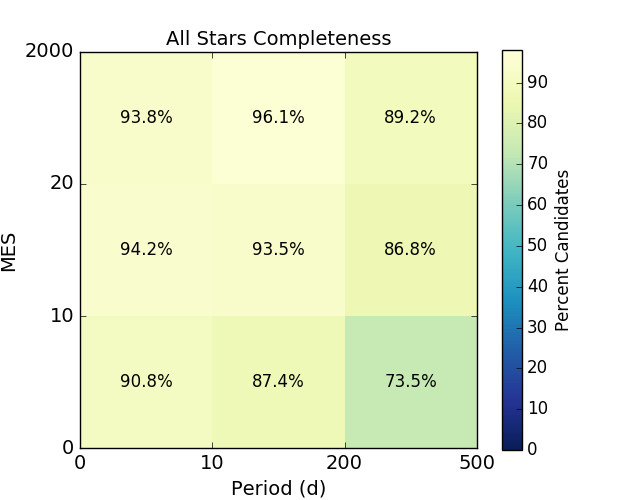
\includegraphics[width=0.9\linewidth]{fig-AllCompletePmes.png}
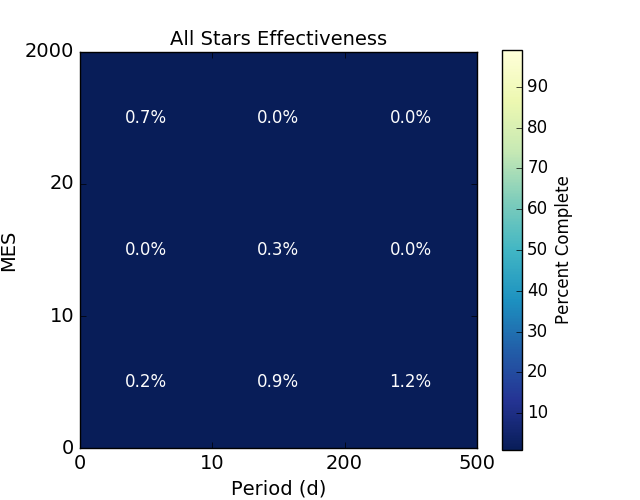
\includegraphics[width=0.9\linewidth]{fig-AllEffect-Pmes.png}
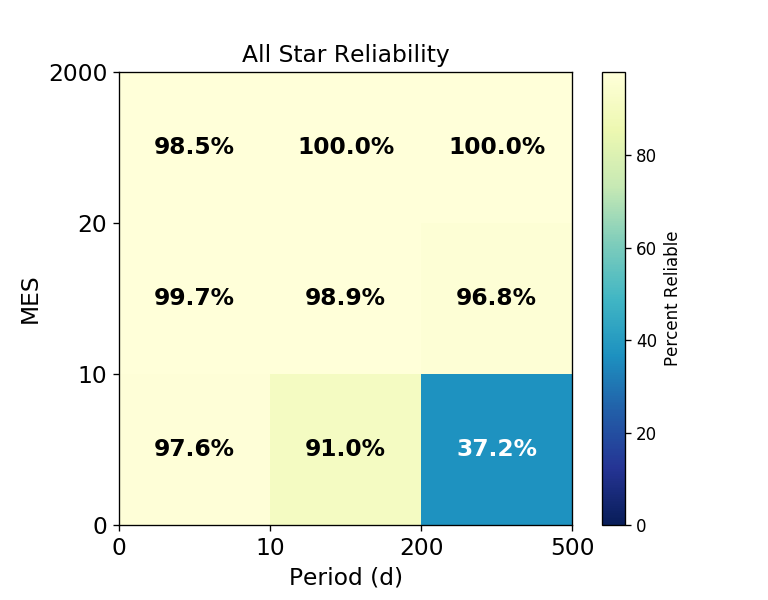
\includegraphics[width=0.9\linewidth]{fig-AllReliabilityPmes.png}
%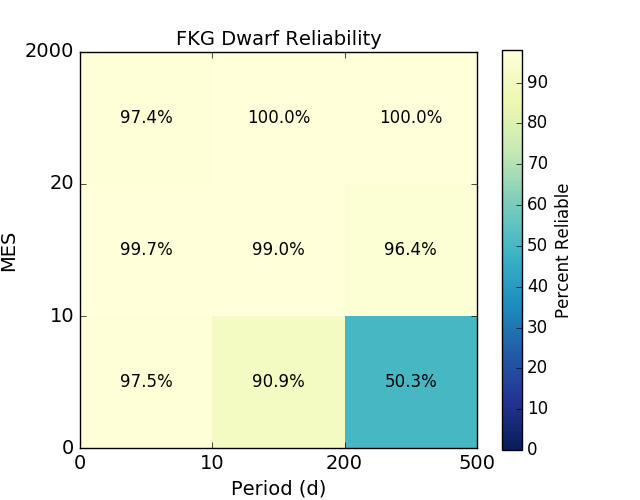
\includegraphics[width=0.48\linewidth]{fig-FgkReliabilityPmes.png}
%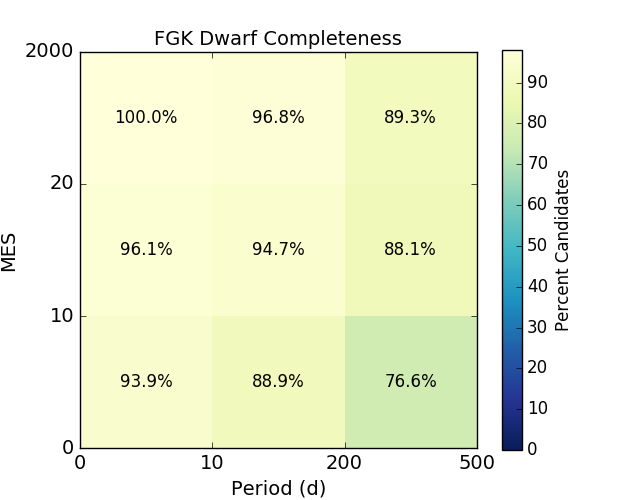
\includegraphics[width=0.48\linewidth]{fig-FgkCompletePmes.png}
\caption{ A coarse binning of the completeness ($C$), in-effectiveness ($1-E$) and reliability ($R$) for different period and MES bins. The effectiveness and reliability are based on the combined \invtce{} and \scrtce{} data sets. Notice that the Robovetter effectiveness at removing these false alarms is incredibly high, but for long periods and low MES the reliability this still results in a low reliability because of the large number of false alarms. }
\label{f:scoregrid}
\end{center}
\end{figure}


%For the later, we use the parameters provided by the supplemental DV fits.  \citet{Christiansen2017} shows that the radii based on the MCMC fits match those of the supplemental DV fits. We do not provided MCMC fits of the entire set of false positives in the \opstce\ set and so cannot use them for our analysis here.

\subsubsection{Completeness}
The completeness of the vetting is measured by determining the fraction of \injtce{s} that are dispositioned as PCs. We discuss here the detection efficiency of the Robovetter, not the Kepler Pipeline (see \S\ref{s:occurates} for a discussion of the Pipeline completeness). Across the entire set of recovered \injtce{s}, periods ranging from 0.5--500\,d, the robovetter recovered \completeness{} per cent. As expected the vetting completeness is higher for transits at shorter periods and higher MES and lower for longer periods and lower MES planets. The right hand column of Figure~\ref{f:1dcompare} shows how the completeness varies with period, expected MES\footnote{Expected MES is the MES the injected transit signal should have had given the noise and the injected depth. See \citet{Christiansen2017} for more details.}, number of transits and duration. The small drop in completeness just short of 90\,days is real and is caused by the odd-even metric (\S\ref{s:oddeven}) confusing true transits for eclipsing binaries.  

Because most planet occurrence rate calculations are performed in period and radius \citep[e.g.][]{Burke2015}, we show the measured completeness binned by period and radius in Figure~\ref{f:prCompleteness}. The plot is linear in period and radius, except for the shortest period planets, in order to emphasize the more interesting long period planets. Planetary radius is not a natural unit to understand the performance of the Robovetter since it convolves the depth of the transit, the noise level of the light curve, and the stellar radius.  At the longest periods the Robovetter more likely fails the largest planets.  When only considering the FGK dwarf stars, this trend is reduced.  These large radii planets are primarily around giant stars, which are notoriously noisy. Thus, they are more likely to be missed. Also, even when only considering the dwarf stars, a larger fraction of the large planets will be around larger, more massive stars. This results in planets with longer transit durations. The Robovetter performs less well for long durations (see Figure~\ref{f:1dcompare}. For more figures showing the effectiveness across different parameters, see \citet{Coughlin2017a}.
%For example, the probability of a planet's single transit overlapping a cadence impacted by image artifacts is higher (\S\ref{s:skye}) or the fit performed by Mars 


\subsubsection{Effectiveness}
The effectiveness of the Robovetter at identifying instrumental and stellar noise is calculated using the union of the \invtce{s} and the \scrtce{s} (see \S\ref{s:relcalc}), after removing the TCEs specified in \S\ref{s:clean}. Across the entire set, the Robovetter removes 99.6 per cent.  Only 119 of the 28,735 simulated false positives are dispositioned by the Robovetter incorrectly (i.e. as a PC).  Unfortunately most of these invPCs and scrPCs fall at long periods and low MES.
Using the 4544 \invtce s and \scrtce s that have periods between 200\,d and 500\,d and MES less than 10, the Robovetter's effectiveness is 98.8 per cent, see Figure~\ref{f:scoregrid}.  Unfortunately, because there are so few candidates at these long periods, this translates to a relatively low reliability.  For detailed plots showing how effectiveness varies with different parameters see \citet{Coughlin2017a}.


\subsubsection{Reliability}
\label{s:reliability}
The reliability is measured according to the method described in \S\ref{s:relcalc} using the effectiveness measured from the combined \scrtce{} and \invtce{} data sets and the number of observed PCs.  If one bins over the entire data sets, the overall reliability of the catalog is 97 per cent. However, as Figure~\ref{f:1dcompare} demonstrates, the reliability for long period, and especially low MES planets is significantly lower.  For periods longer than 200\,d and MES less than 10, the reliability of the catalog is approximately 37 per cent, i.e. 6 out of 10 PCs are actually caused by noise. As with completeness, we plot the reliability as a function of period and planet radius in Figure~\ref{f:prReliability}. As expected the least reliable planets are at long periods and have radii less than 4 earth radii. 

The error in the reliability is likely dominated by how well the false alarms in the \scrtce{} and \invtce{} sets match the false alarms in the \opstce{} data set. See \S\ref{s:simularity} for further discussion on their similarity.  One way to get an handle on the uncertainty this creates, we calculate reliability in three different ways for the long period (200--500\,d), low MES ($<10$) \opstce{s}.  First, we use only the \invtce{s} to measure the effectiveness at removing false alarms. This results in a lower reliability, namely R$=24$~per cent and $E=98.5$~per cent. Second, we use only the \scrtce{s} to measure the effectiveness. This results in a higher reliability, R$=51$~per cent and E=$99.1$~per cent. Third, we select, at random, half of the the combined population of false alarms (\scrtce{} and \invtce{}) and calculate the reliability. After doing this random selection 100 times, we obtained R$=38$~per cent with a standard deviation of 8~percent and the distribution appears basically Gaussian in shape.  

The Robovetter is less effective at removing the false alarms produced by inversion than those by scrambling the data. Inversion finds false alarms at 372\,d frequently caused by image artifacts.  Scrambling is under-populated by these false alarms. And since these types of false alarms are the most difficult to eliminate, it is not surprising that the reliability measured by inversion is worse than when measured by scrambling.  The truth likely lies somewhere in between. We encourage users of these data sets to consider ways to optimize this reliability measurements, and the error budget associated with them, when doing occurrence rate calculations. 


\begin{figure*}[ht]
 \begin{center}
  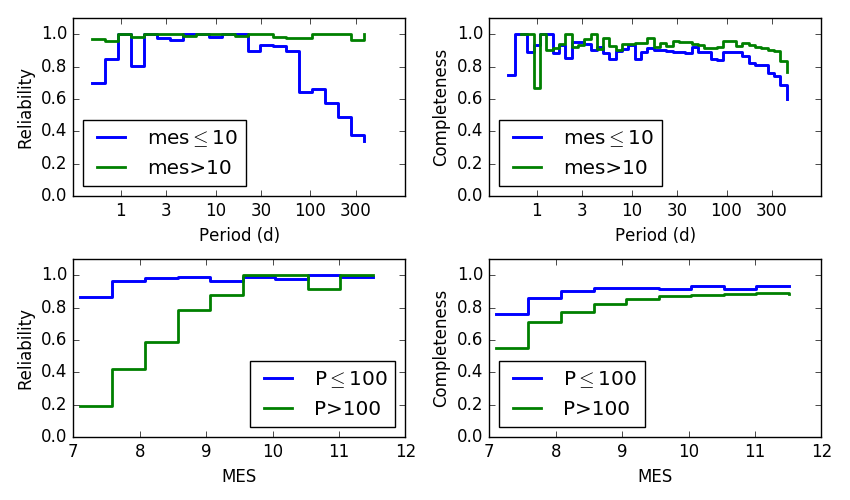
\includegraphics[width=0.93\linewidth]{fig-compRel1D-PerMes.png}
  \caption{ The completeness (right) and reliability (left) of the DR25 catalog plotted for Period, MES, number of transits and duration. In each case the blue line is for those with MES$\leq$10 or periods $\leq$ 100\,d. The green line shows the completeness or reliability for the rest of the population. See the legend for each figure. }
  \label{f:1dcompare}
 \end{center}
 \end{figure*}

\begin{figure*}[ht]
\begin{center}
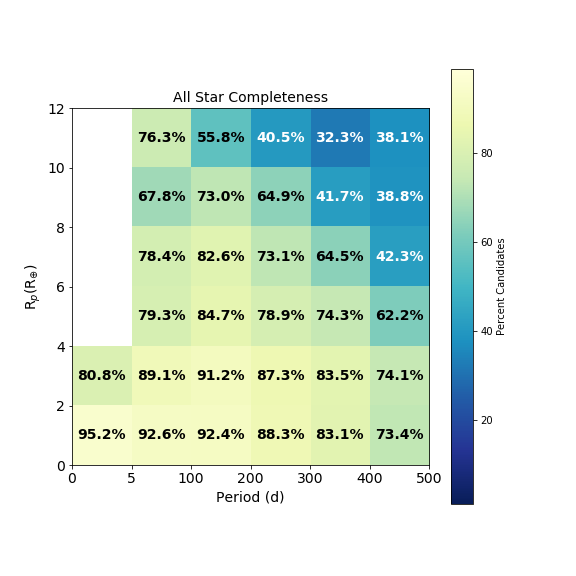
\includegraphics[width=0.45\linewidth]{fig-AllCompletePR.png}
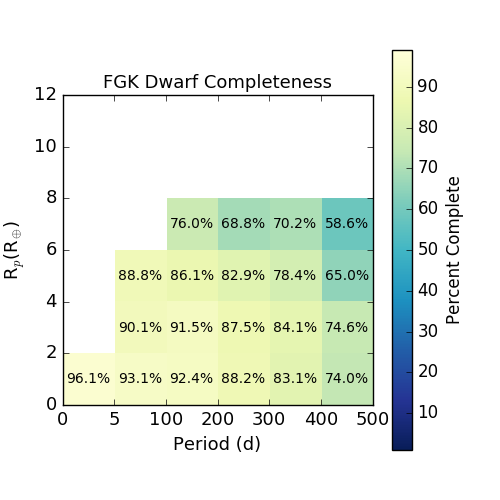
\includegraphics[width=0.45\linewidth]{fig-FgkCompletePR.png}
\caption{The Robovetter completeness binned by period and planet radius for all stars (left) and for only FGK dwarf stars (right). Bins with fewer than 10 \injtce{s} are not plotted.}
\label{f:prCompleteness}
\end{center}
\end{figure*}

\begin{figure*}[ht]
\begin{center}
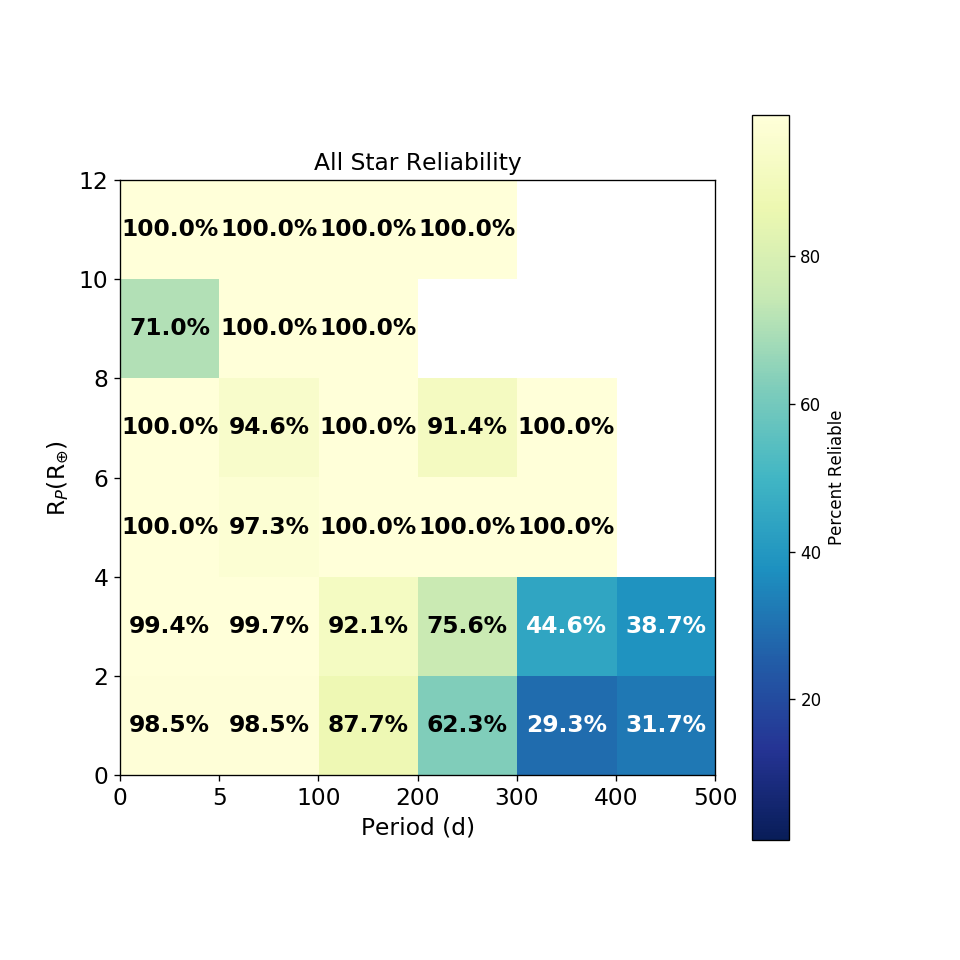
\includegraphics[width=0.45\linewidth]{fig-AllReliabilityPR.png}
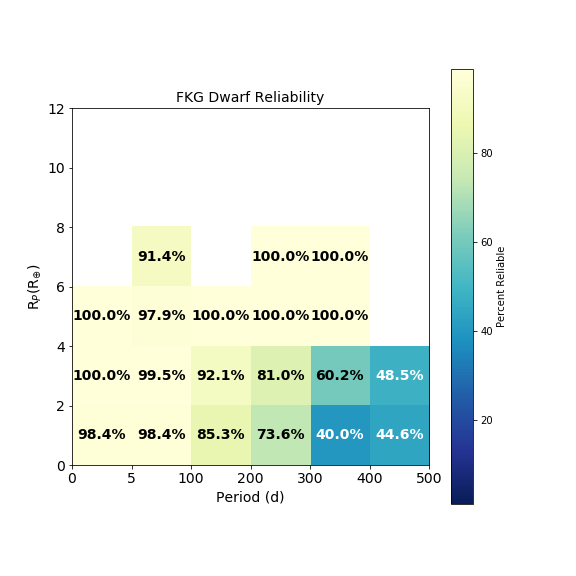
\includegraphics[width=0.45\linewidth]{fig-FgkReliabilityPR.png}
\caption{A 2D binning of the candidate catalog reliability for period and planet radius for all stars (left) and for the FGK dwarf stars (right). Bins with fewer than 3 candidates or fewer than 20 simulated false alarms (from \invtce{} and \scrtce{}) are not plotted.}
\label{f:prReliability}
\end{center}
\end{figure*}



\subsubsection{High Reliability Using the Disposition Score}
\label{s:crscores}

The disposition scores discussed in \S\ref{s:scores} can be used to select a more reliable, though more incomplete, sample of planet candidates. In Figure~\ref{score-fig-2} we show the distribution of the score values for of the PCs and FPs for each of the observed, inverted, scrambled, and on-target planet injection populations. (Note that the inverted and scrambled populations have been cleaned as discussed in \S\ref{s:clean}). For all populations, the PC distribution tends to cluster near a score of 1.0 with a tail that extends towards lower score values. Lower MES values tend to have a greater proportion of lower score values. Similarly, the vast majority of FPs have a score of 0.0, with only a small fraction extending towards higher score values (note the y-axis for the FPs is logarithmic, while the y-axis for PCs is linear.) Comparing between the populations, the on-target planet injections have a greater concentration of score values towards 0.5 for both the PCs and FPs than other populations. Both the inverted and scrambled populations have very few PCs near high score values. We can exploit the relative distribution of PC and FP score values for the different populations to improve the completeness and reliability of the catalog.

\begin{figure*}[ht]
\centering
\begin{tabular}{cc}
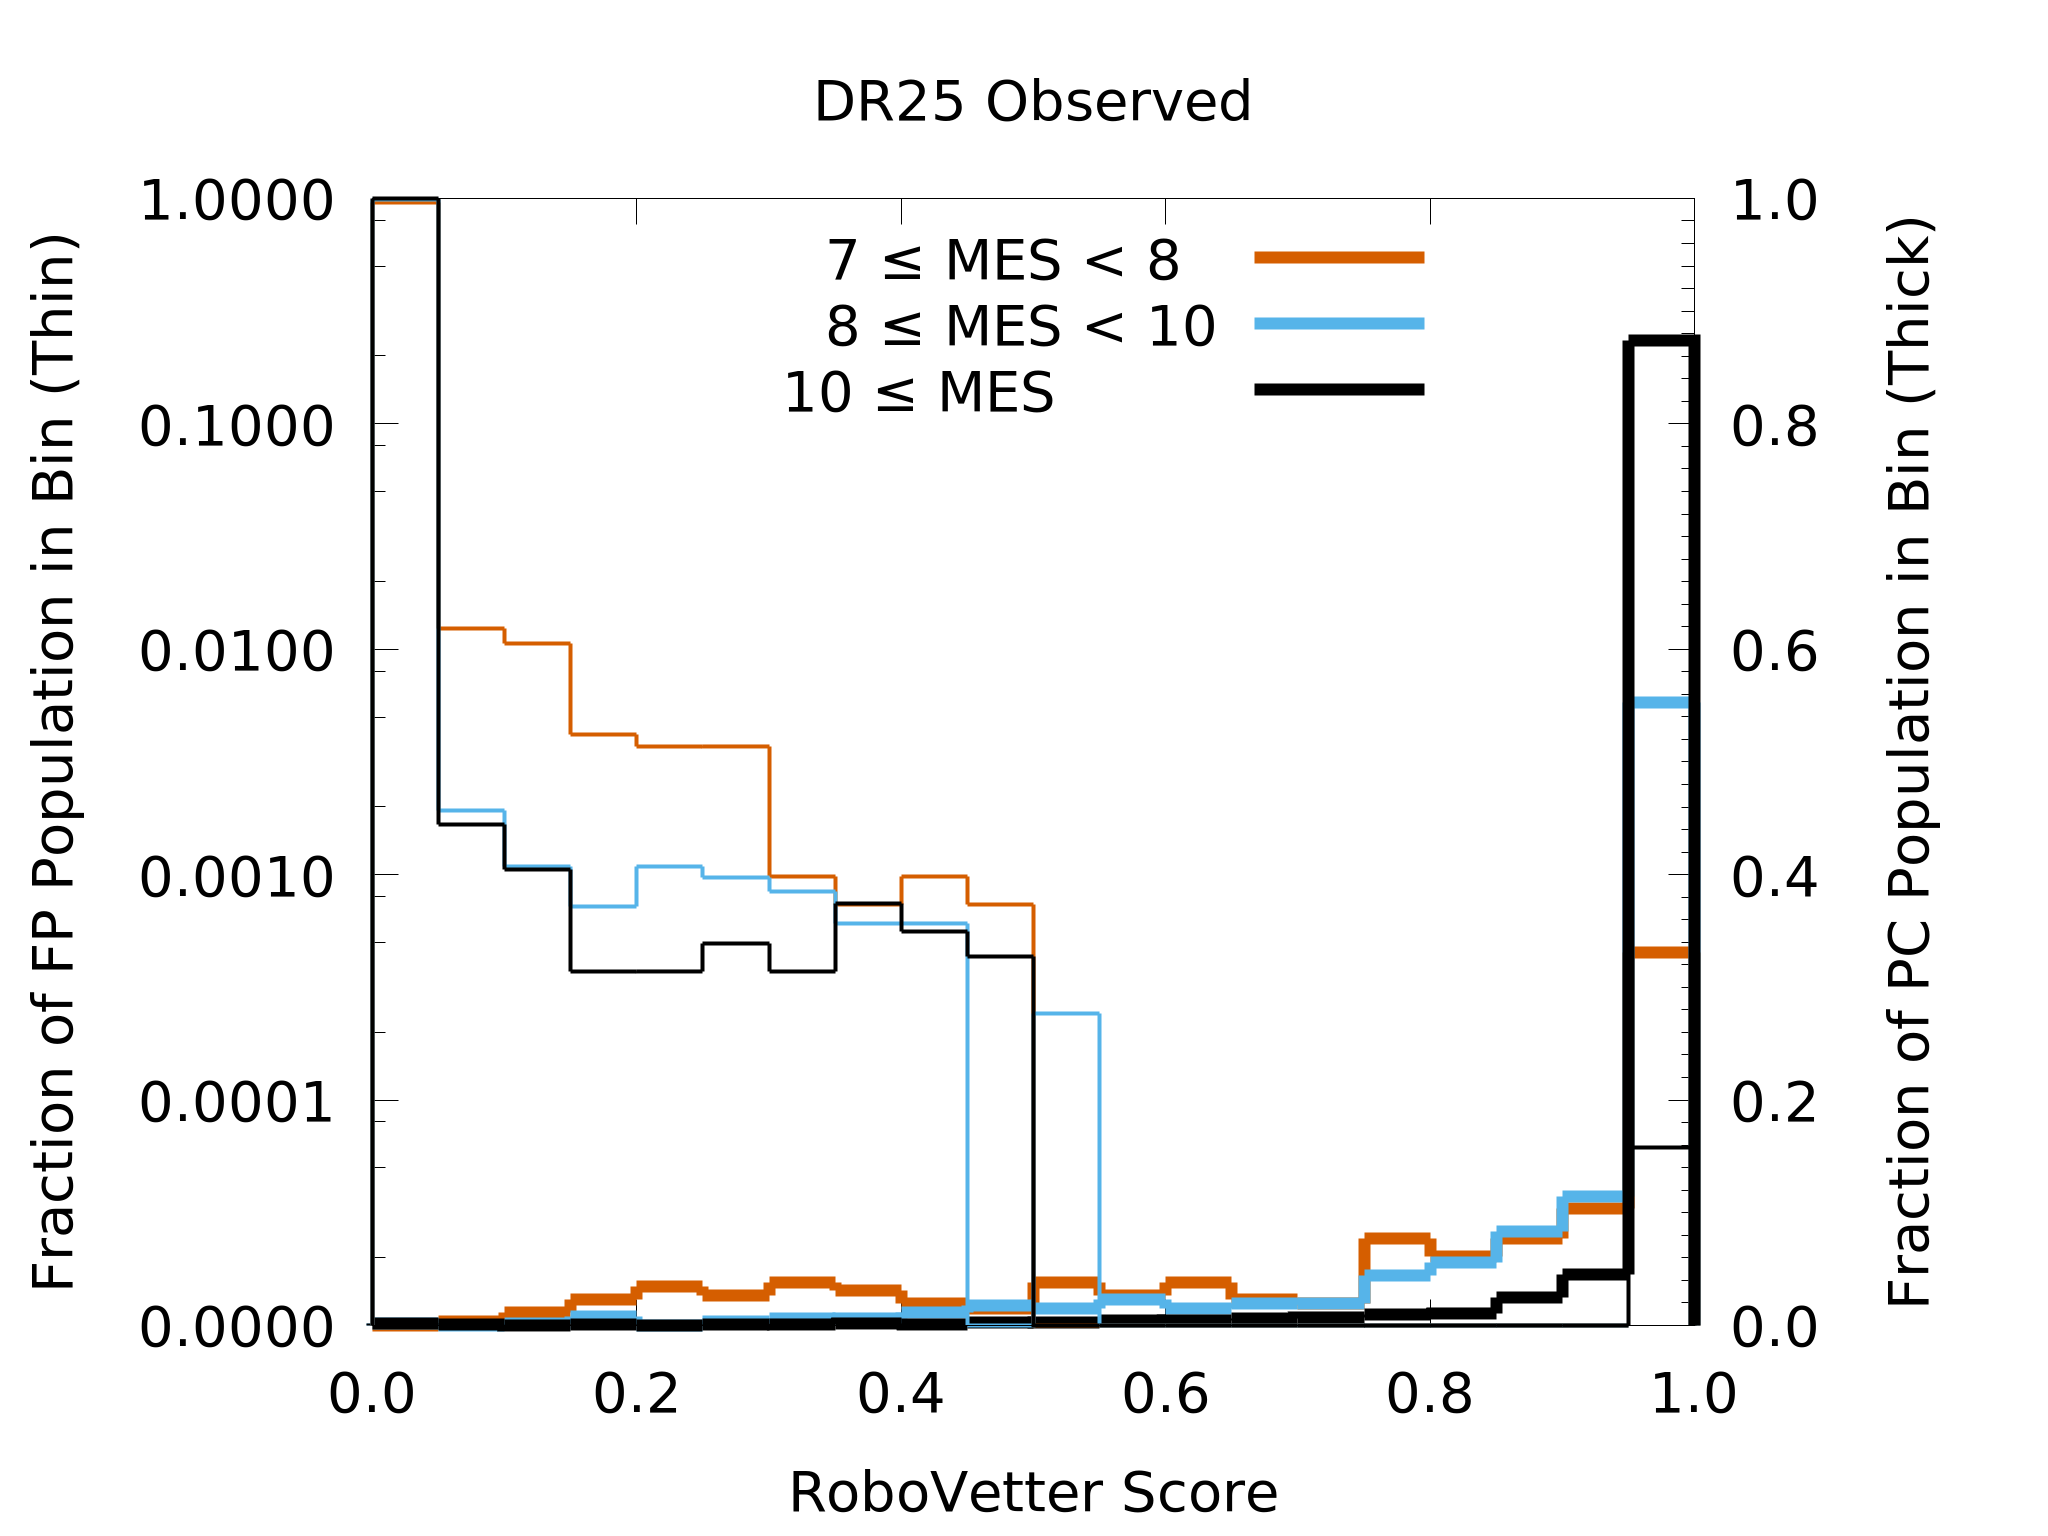
\includegraphics[width=0.48\linewidth]{Scores-OBS.png} &
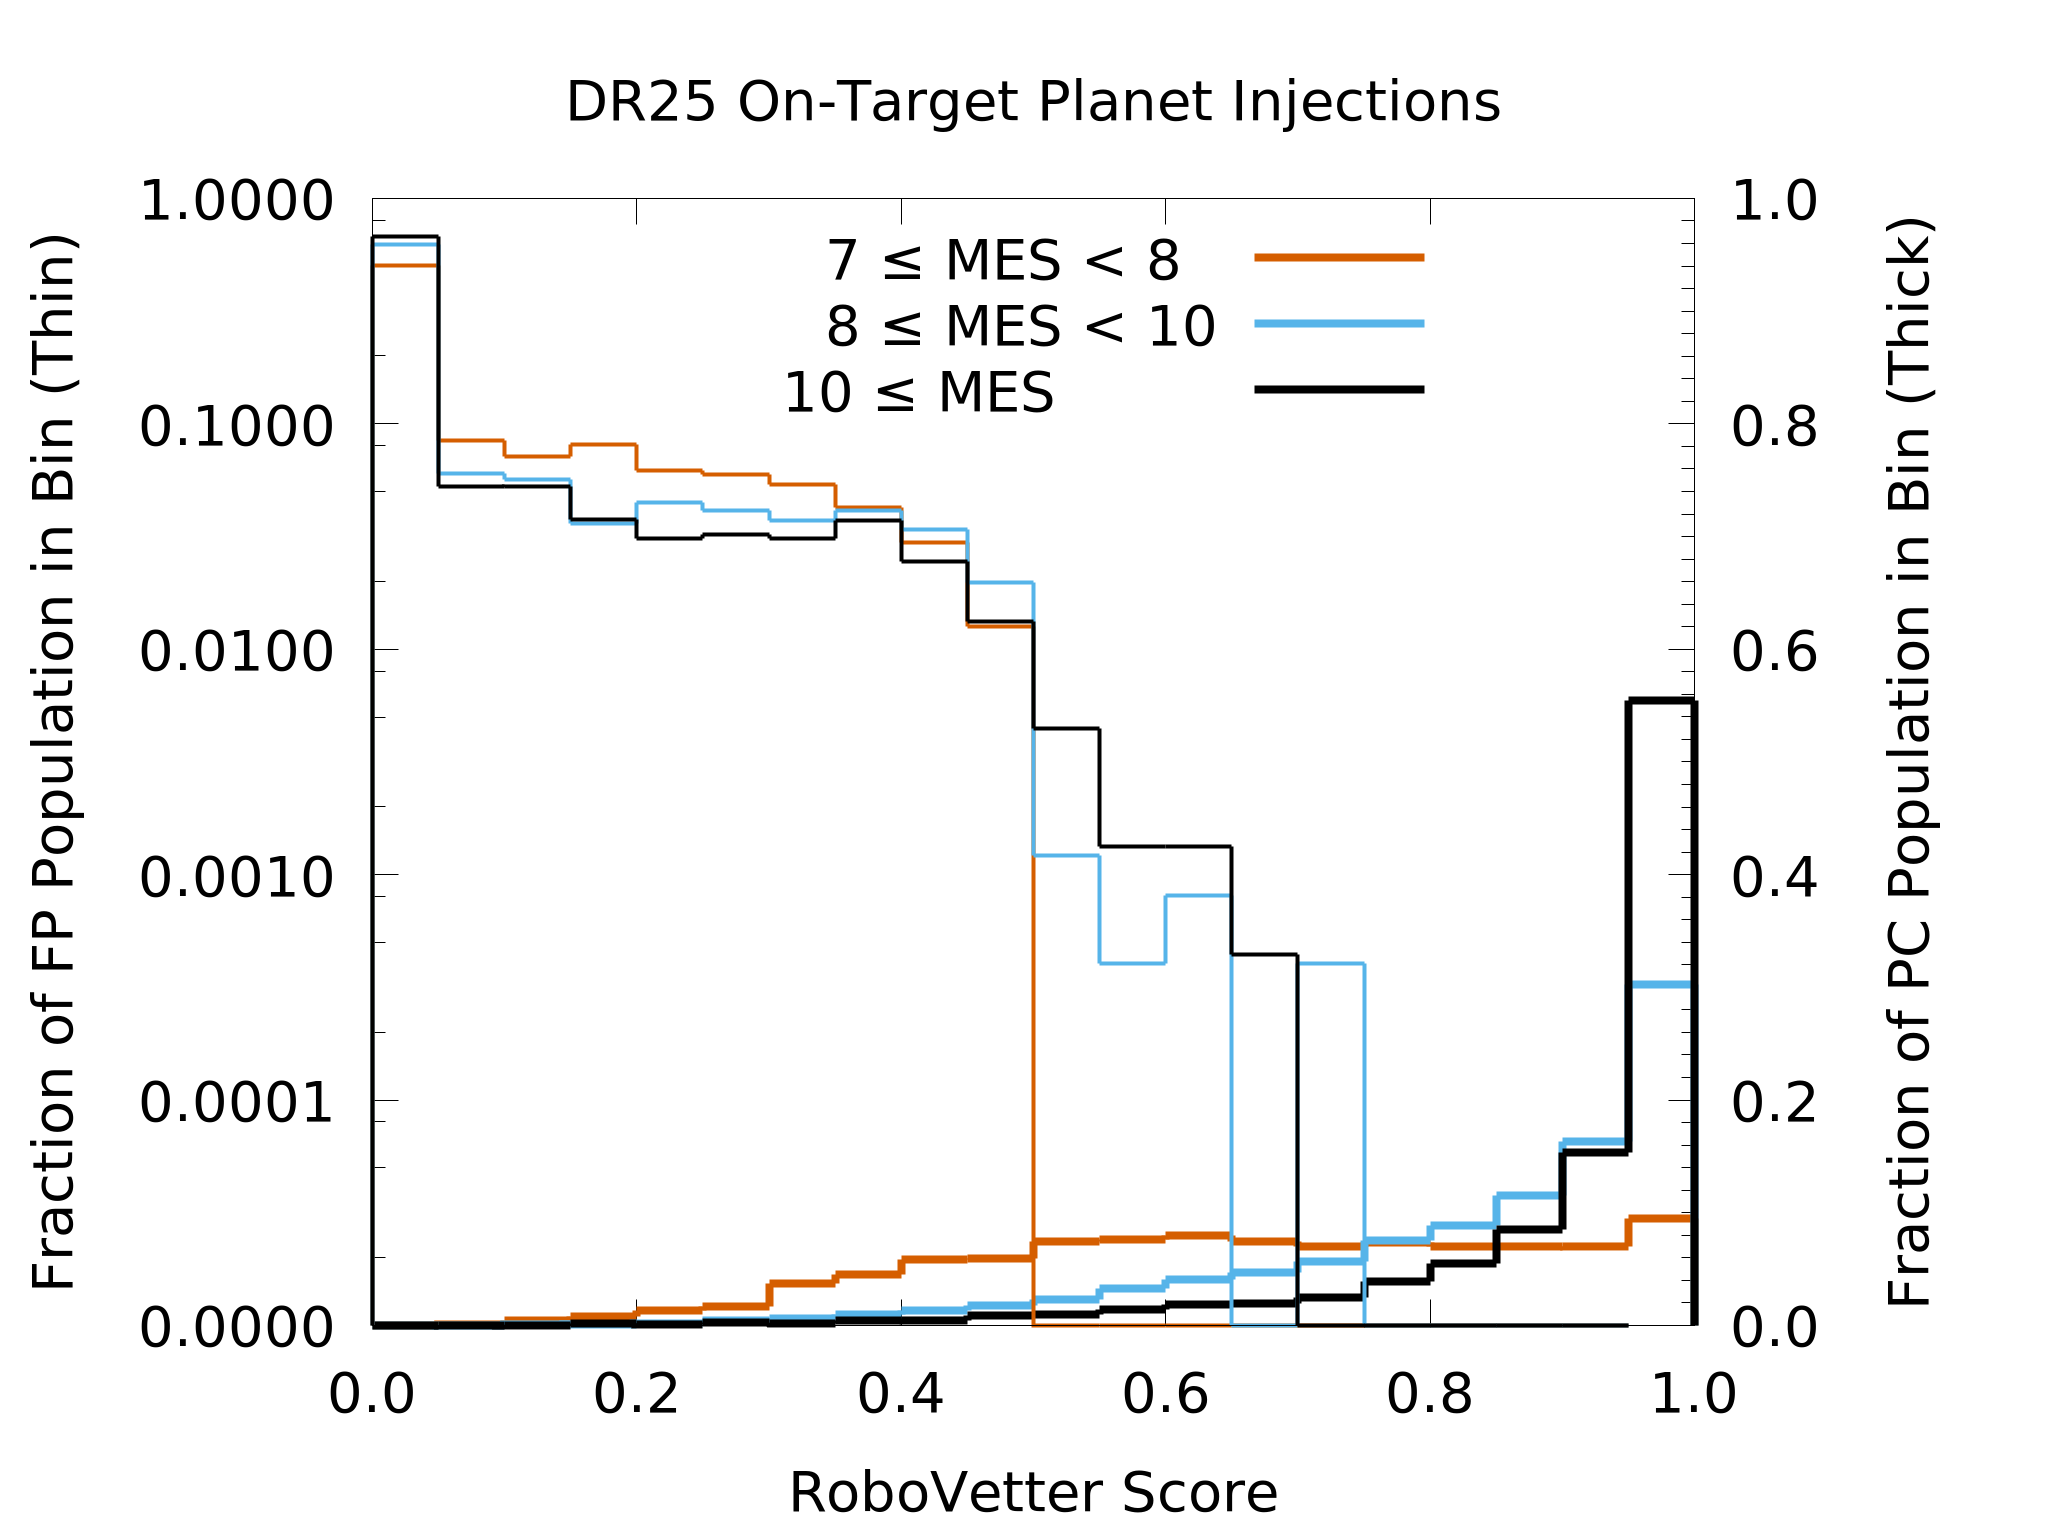
\includegraphics[width=0.48\linewidth]{Scores-INJ1.png} \\
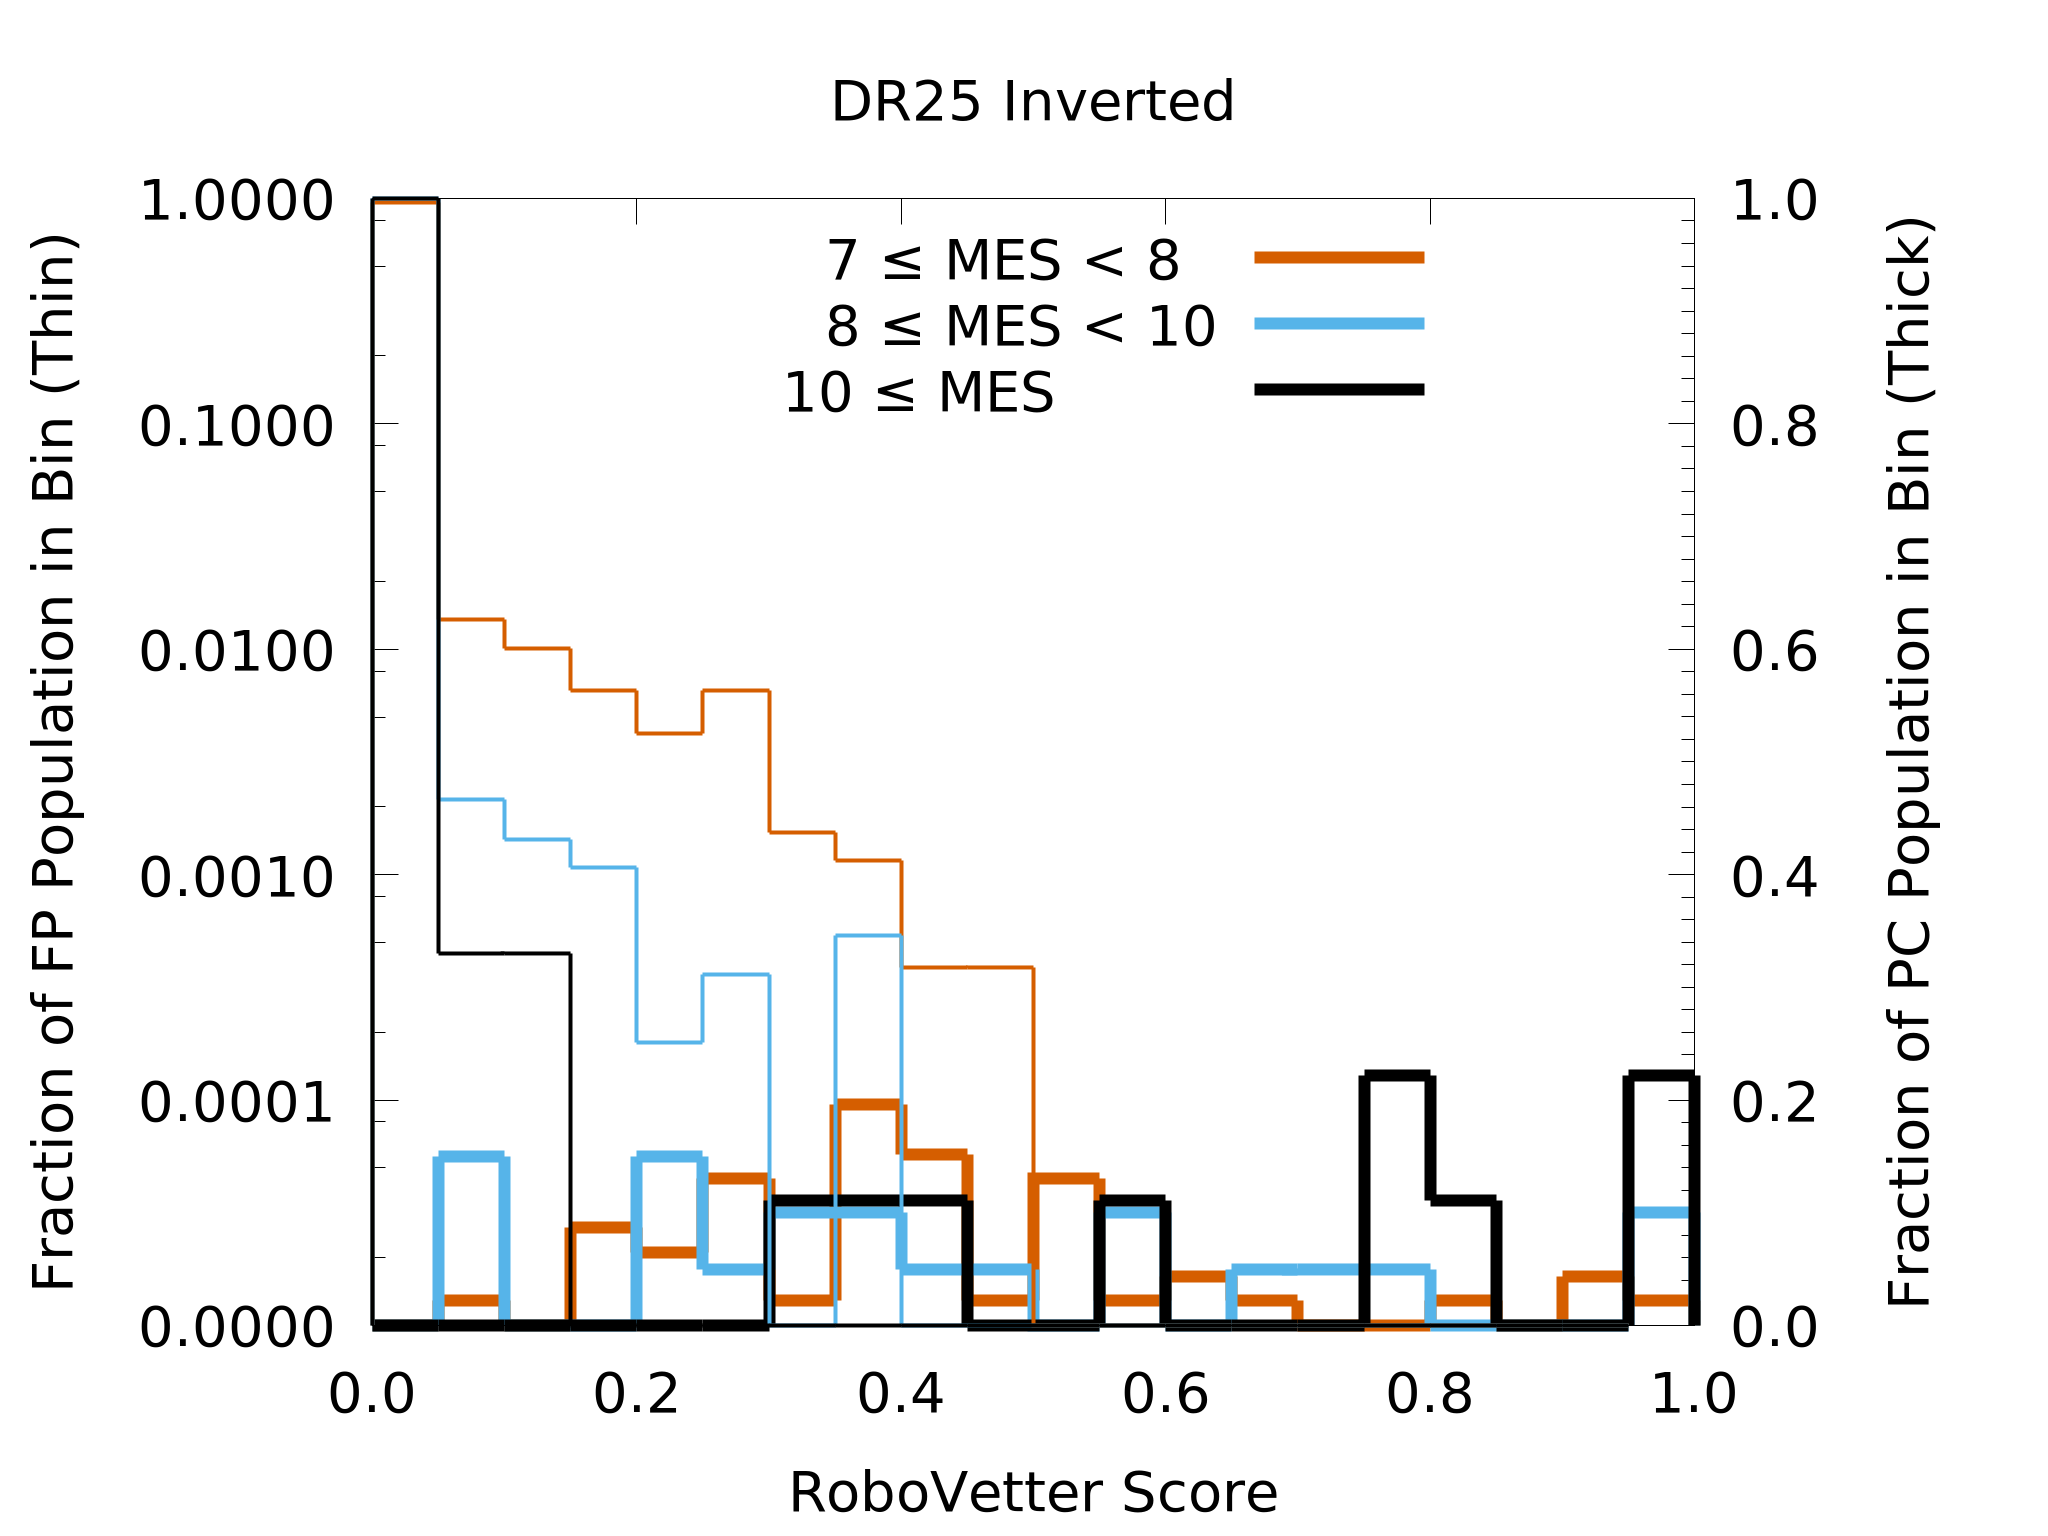
\includegraphics[width=0.48\linewidth]{Scores-INV.png} &
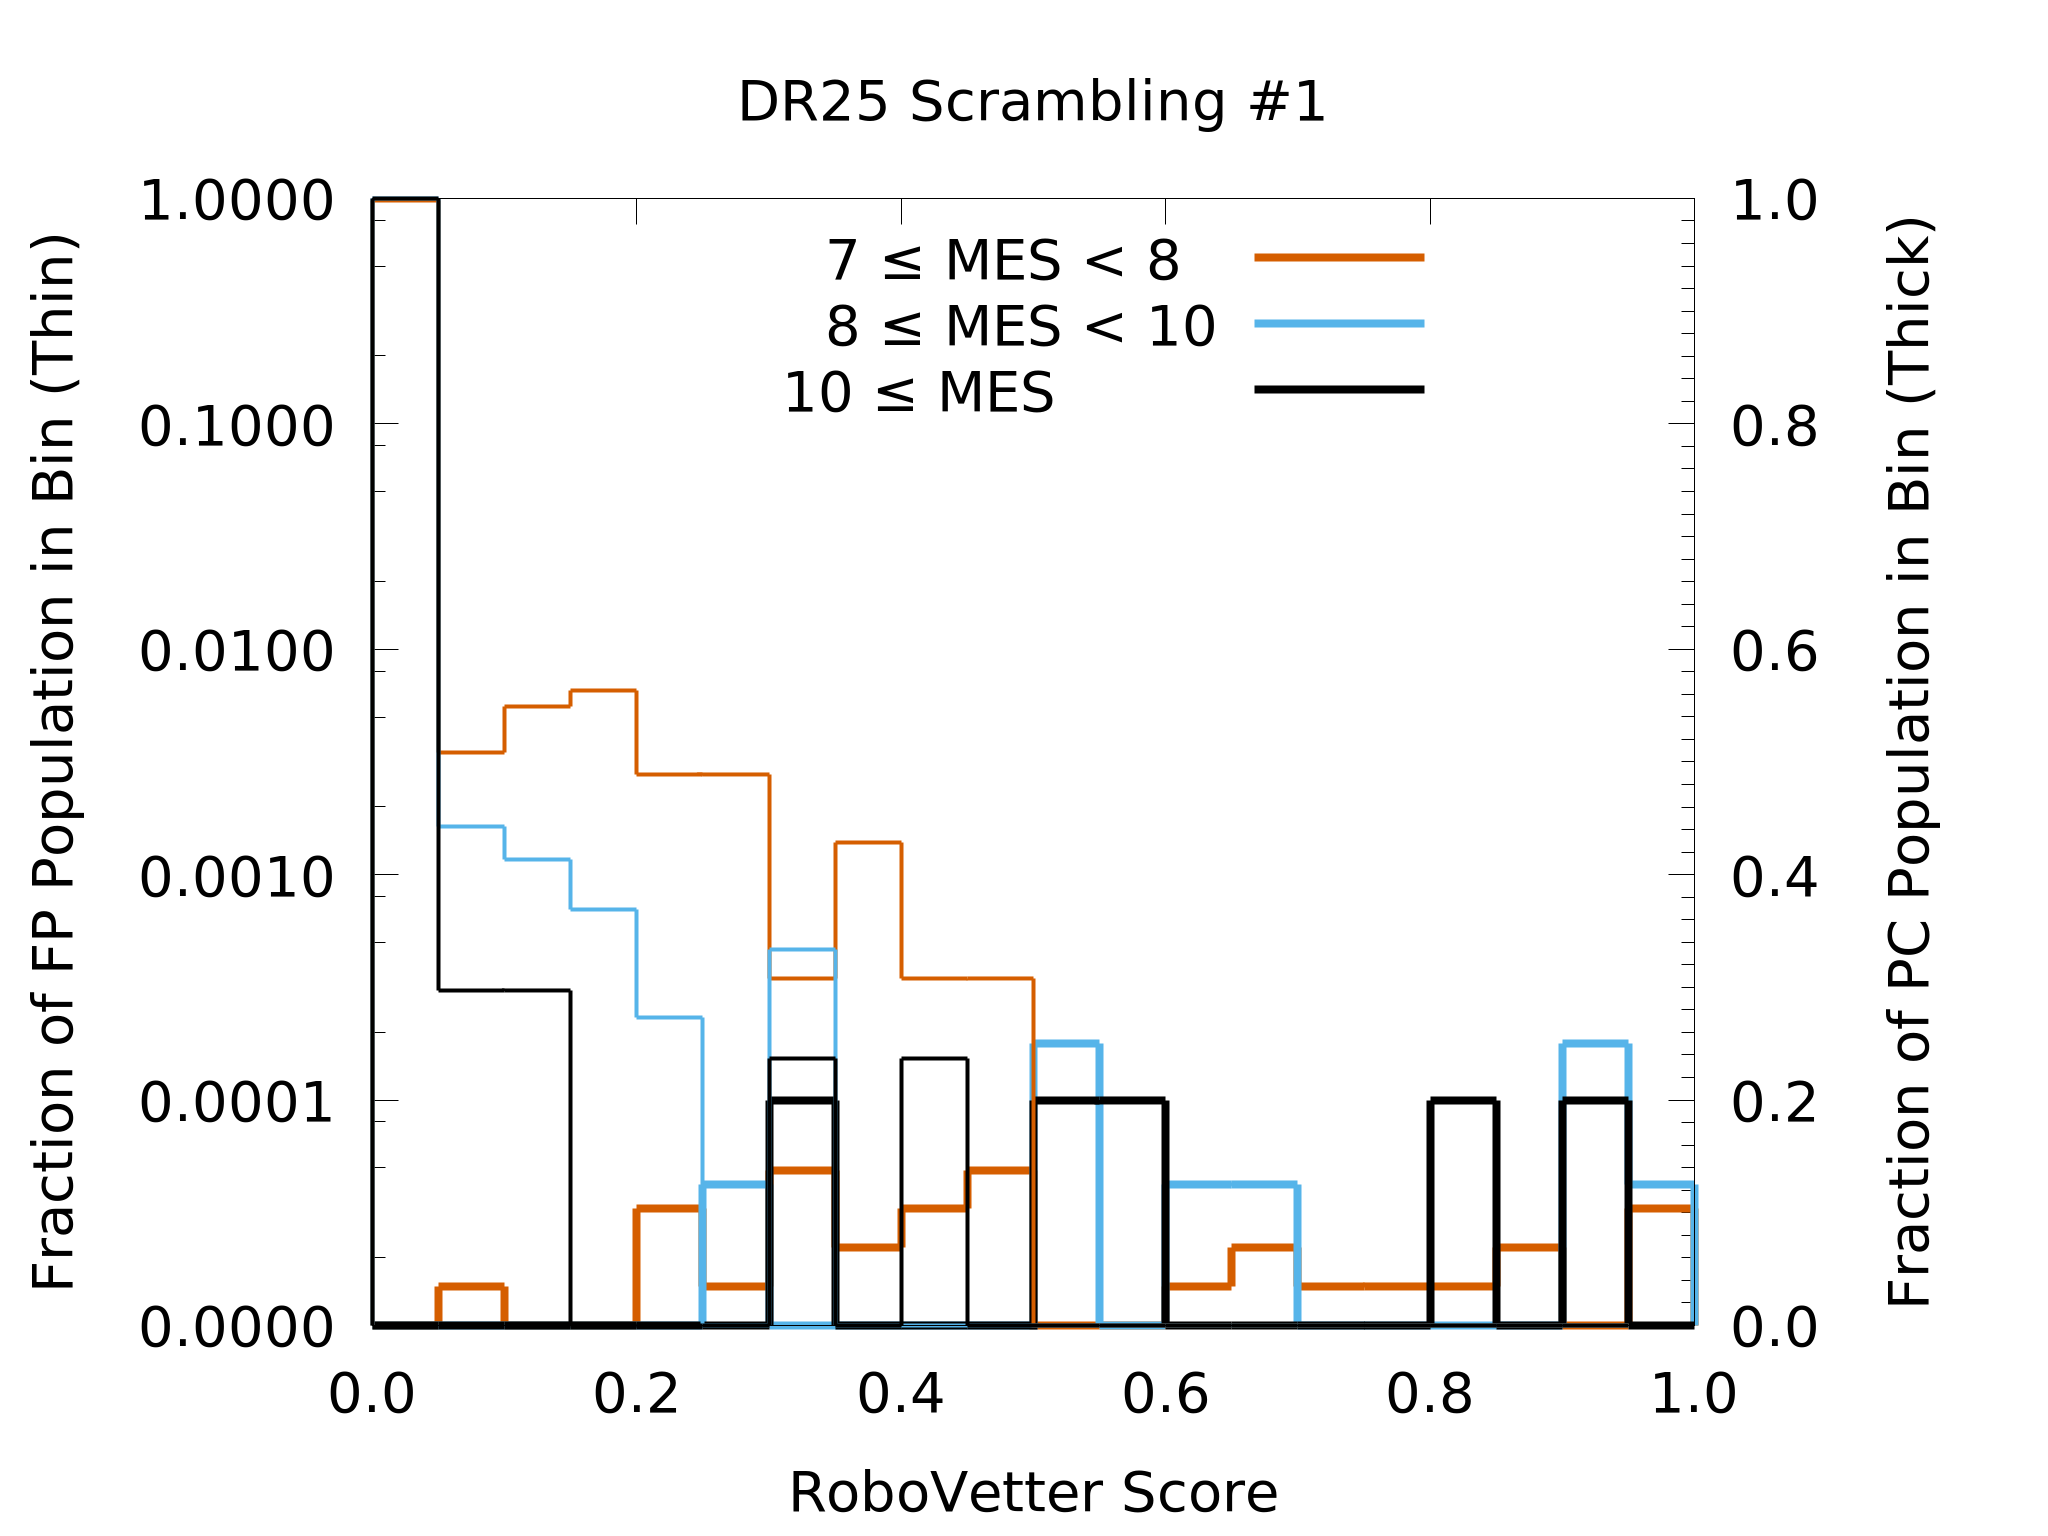
\includegraphics[width=0.48\linewidth]{Scores-SCR1.png} \\
\end{tabular}
\caption{Plots of the score distribution of PCs (thick lines, right y-axis) and FPs (thin lines, left y-axis, logarithmic scaling) for the observed (top-right), on-target planet (top-left), inverted (bottom-left), and scrambled (bottom-right) TCEs.}
\label{score-fig-2}
\end{figure*}

At the top of Figure~\ref{f:adjscore} we show how the completeness and reliability of the catalog vary for different cuts on the disposition score for MES$<$10 and periods between 200 and 500 days. Notice that the effectiveness of the Robovetter increases as expected as the score threshold is increased. The reliability values also depend on the number of observed PCs that remain, which is why reliability does not change in step with the effectiveness. Selecting PCs by choosing those with a disposition score above 0.6 will yield an 85 per cent reliability with a completeness that is still above 50 per cent. Doing a score cut in this way causes a few \opstce{s} which are formally called an FP to be promoted to a PC. An FP with a high score occurs when a TCE marginally fails a single metric.  

It is interesting to note that the number of inferred candidates, i.e. the number of candidates after accounting for the Robovetter completeness and catalog reliability, does not change significantly with the score cut. In the bottom plot of Figure~\ref{f:adjscore} we plot both the observed number of PCs and the corrected number of PCs.  The correction is done by taking the number of PCs and multiplying by the reliability and dividing by the completeness.  The error bars only include the Poisson counting error in the number of observed PCs and does not include errors in the measure completeness or reliability. The corrected number of PCs only varies by approximately 1$\sigma$ regardless of the score cut used.   

\begin{figure}[ht]
 \begin{center}
 \begin{tabular}{c}
  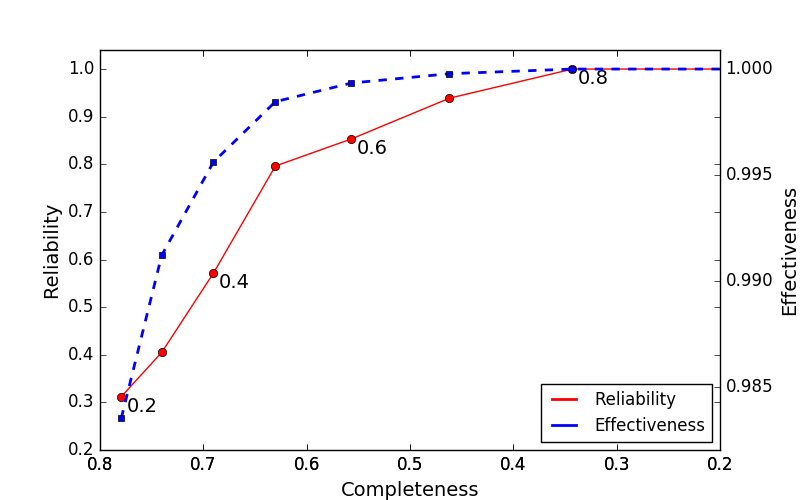
\includegraphics[width=1.0\linewidth]{fig-CRadjustScore-DR25.png} \\
  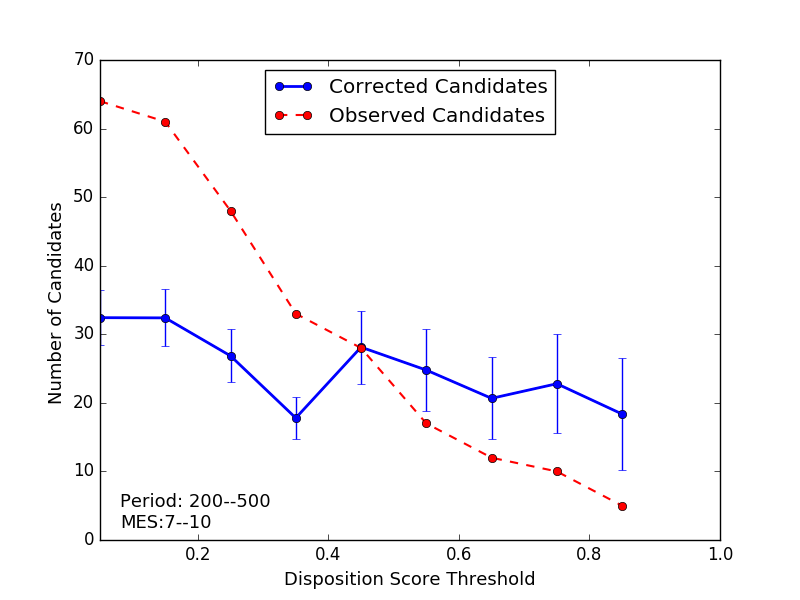
\includegraphics[width=1.0\linewidth]{fig-varyScoreNcandidatesBox2.png}
  \end{tabular}
  \caption{\label{f:adjscore}[Top] The reliability (red) and effectiveness (blue) of the MES$\leq$10 and periods between 200 and 500\,d PCs that results when using a disposition score threshold to select the PCs.  [Bottom] The number of PCs in the same period and MES space when making a cut on different disposition scores is plotted in red.  The blue line corrects the number of candidates for the completeness and reliability. The error bars only reflect a Poisson error based on the number of observed planet candidates.}
 \end{center}
 \end{figure}


